\section{Dispersion Relations for Concrete Graph Geometries} \label{sec:ScalarExamples}
In this section we provide examples to demonstrate how the spectrum $\sigma=\sigma\bracs{-\laplacian_{\upsilon}}$ is obtained via the analysis of the $M$-matrix for the quantum graph problem \eqref{eq:SingularWaveEqnQGProblem}.
The examples are chosen to highlight the methodology and some of the remarks discussed in sections \ref{sec:QuantumGraphs} and \ref{sec:ScalarDiscussion}.
In each of these examples we will encounter a number of terms with similar forms, so to avoid repetition we define these quantities here.
Let $a\in\bracs{0,1}$ and define
\begin{align} \label{eq:SE-CommonTrigFns}
	s_a\bracs{\omega} &= \sin\bracs{a\omega}, \quad 
	c_a\bracs{\omega} = \cos\bracs{a\omega}, \quad
	\tilde{s}_a\bracs{\omega} = \sin\bracs{(1-a)\omega}, \quad 
	\tilde{c}_a\bracs{\omega} = \cos\bracs{(1-a)\omega}.
\end{align}
The quantities in \eqref{eq:SE-CommonTrigFns} are $\omega$-dependent, however throughout this section we will suppress this dependency unless providing important formulae. 

\subsection{One-dimensional chain} \label{ssec:Example1DLoop}
We begin with the simplest example, a chain of vertices periodic in one direction, to demonstrate how one takes the period graph of a physical singular-structure and employs proposition \ref{prop:M-MatrixEntries} to construct the $M$-matrix and extract the spectral information.
We also use the simplicity of this example to highlight the necessity of splitting edges via the introduction of artificial vertices to remove loops and edge-lengths that are rationally-related, to compliment section \ref{ssec:ArtificialVertices}.

Consider the graph $\hat{\graph}$ periodic in one direction in $\reals\times\sqbracs{0,1}$, with vertices $v_j = \bracs{j + \recip{2}, 0}^\top$ and edges $I_{j\bracs{j+1}}, \ j\in\integers$.
Since $\hat{\graph}$ is parallel to- and periodic in the $x_1$-direction, the period cell lies in $S^1$ and the quasi-momentum $\qm\in\left[-\pi,\pi\right)$ is scalar\footnote{One can simply set $\qm_2=0$ in \eqref{eq:SingularWaveEqnQGProblem} when constructing the $\qm_{jk}$ to account for the lack of periodicity in $x_2$.}.
Place identical coupling constants at each vertex, with $\alpha_j = \alpha_1>0 \ \forall v_j\in\vertSet$.
The period graph $\graph$ of $\hat{\graph}$ consists of a single vertex $v$ (without loss of generality placed at the origin) with a looping edge $I$ of length 1, with quasi-momentum $\qm_I=\qm$ on $I$ and coupling constant $\alpha_1$ at $v$.
We must introduce an artificial vertex (section \ref{ssec:ArtificialVertices}) to break the loop $I$ into two edges with irrationally-related edge lengths, producing a new metric graph $\graph^*=\bracs{\vertSet, \edgeSet}$ (on which \eqref{eq:SingularWaveEqnQGProblem} is posed) with
\begin{align*}
	\vertSet = \clbracs{ v_1 , v_2 }, \quad \edgeSet = \clbracs{ I_{12}, I_{21} },
	&\qquad \abs{I_{12}} = a, \quad \abs{I_{21}} = 1-a,  \\
	\alpha_1 >0, \quad \alpha_2 = 0,
	&\qquad \qm_{12} = \qm_{21} = \qm,
\end{align*}
where $a$ and $1-a$ are irrationally related --- taking $a = \recip{\sqrt{2}}$ would suffice, for example.
The process of moving from $\hat{\graph}$ through $\graph$ to $\graph^*$ is illustrated in figure \ref{fig:Diagram_1DExample}.
\begin{figure}[t!]
	\centering
	\begin{subfigure}[t]{0.3\textwidth}
		\centering
		\includegraphics[scale=2]{Diagram_1DLineGraph.pdf}
		\caption[]{\label{fig:Diagram_1DLineGraph} The graph $\hat{\graph}$, periodic in one dimension, consisting of integer-spaced vertices.}
	\end{subfigure}
	~
	\begin{subfigure}[t]{0.3\textwidth}
		\centering
		\includegraphics[scale=2]{Diagram_1DLineQuantumGraph.pdf}
		\caption[]{\label{fig:Diagram_1DLineQuantumGraph} The metric graph corresponding to the period graph $\graph$, containing one (looping) edge of length 1}
	\end{subfigure}
	~
	\begin{subfigure}[t]{0.3\textwidth}
		\centering
		\includegraphics[scale=2]{Diagram_1DLineComputationGraph.pdf}	
		\caption[]{\label{fig:Diagram_1DLineComputationGraph} The metric graph $\graph^*$ obtained by the introduction of a dummy vertex $v_2$, which has coupling constant 0.}
	\end{subfigure}
	\caption[The 1D chain graph studied in the example of section \ref{ssec:Example1DLoop}.]{\label{fig:Diagram_1DExample} The graphs $\hat{\graph}$, $\graph$, and $\graph^*$.}
\end{figure} \newline

Using proposition \ref{prop:M-MatrixEntries} and corollary \ref{cory:M-MatrixEntriesNoPoles} we find that
\begin{align*}
	\mathfrak{M}_{\qm} = 
	\begin{pmatrix}[1.75]
		-\omega c_a \tilde{s}_a - \omega s_a \tilde{c}_{a} + \omega^2\alpha_1 s_a \tilde{s}_a &
		\omega e^{\rmi\qm a} \tilde{s}_a + \omega e^{-\rmi\qm(1-a)} s_a \\
		\omega e^{-\rmi\qm a} \tilde{s}_a + \omega e^{\rmi\qm(1-a)} s_a &
		-\omega c_a \tilde{s}_a - \omega s_a \tilde{c}_a
	\end{pmatrix},
	\qquad
	H^{(2)} = s_a \tilde{s}_a,\\
\end{align*}
using the notation \eqref{eq:SE-CommonTrigFns}.
Since $\graph^*$ is a chain graph with only two vertices, it is easy enough to compute $\det\mathfrak{M}_{\qm}$ and solve \eqref{eq:QGDetSolveCondition} analytically, yielding
\begin{align} \label{eq:1DChainDetEqual0}
	0 = 2\omega^2 s_a\bracs{\omega} \tilde{s}_a\bracs{\omega} \bracs{ \cos\omega - \frac{\omega\alpha_1}{2}\sin\omega - \cos\qm }.
\end{align}
Notice that the factor in front of the brackets in \eqref{eq:1DChainDetEqual0} is $2\omega^2 H^{(2)}\bracs{\omega^2}$, so is zero at $\omega=0$ and at the roots of $H^{(2)}$.
Let us define $\Xi\bracs{\qm,\omega} = \cos\omega - \frac{\omega\alpha_1}{2}\sin\omega - \cos\qm$.
Since $\cos\qm$ attains every value in $\sqbracs{-1,1}$ for $\qm\in\left[-\pi,\pi\right)$, the bracketed term in \eqref{eq:1DChainDetEqual0} implies that any $\omega$ satisfying
\begin{align*}
	-1 \leq \cos\omega - \frac{\omega\alpha_1}{2}\sin\omega \leq 1,
\end{align*}
is part of the spectrum of \eqref{eq:SingularWaveEqnQGProblem}.

We now consider solutions of \eqref{eq:1DChainDetEqual0} that are also zeros of $H^{(2)}$ --- let $\omega_0$ denote one of these values, so $\omega_0\in\clbracs{\frac{n\pi}{a}, \frac{n\pi}{1-a} \setVert n\in\naturals }$.
The eigenvalue branches of $\mathfrak{M}_{\qm}$ can be computed,
\begin{align*}
	\widetilde{\beta}_{\pm, \qm}\bracs{\omega^2} &= -\omega\sin\omega + \frac{\omega^2\alpha_1}{2}s_a \tilde{s}_a \pm \omega\sqrt{ \sin^2\omega + \frac{\omega^2\alpha_1^2}{4}s_a^2 \tilde{s}_a^2 - 2s_a \tilde{s}_a\bracs{\cos\omega-\cos\qm} },
\end{align*}
however only $\widetilde{\beta}_{+, \qm}\bracs{\omega_0^2}=0$.
As such, $\omega_0$ is part of the spectrum of \eqref{eq:SingularWaveEqnQGProblem} when
\begin{align*}
	\lim_{\omega\rightarrow\omega_0}\bracs{ H^{(2)}\bracs{\omega^2} }^{-1}\widetilde{\beta}\bracs{\omega^2}_{+} = 0,
\end{align*}
which (after applying L'h\^{o}spital's rule) only occurs when
\begin{align*}
	\exists\qm_0\in\left[-\pi,\pi\right) \text{ s.t. } \cos\omega_0 - \frac{\omega_0\alpha_1}{2}\sin\omega_0 - \cos\qm_0 = 0,
\end{align*}
that is precisely when there is some $\qm_0$ such that $\Xi\bracs{\qm_0,\omega_0}=0$.
Therefore, the spectrum of \eqref{eq:SingularWaveEqnQGProblem} is fully described by those $\omega$ satisfying
\begin{align*}
	-1 \leq \cos\omega - \frac{\omega\alpha_1}{2}\sin\omega \leq 1.
\end{align*}
We remark here that in the notation of proposition \ref{prop:MMatrixDetForm} and corollary \ref{cory:ScalarSetInclusions}, $F\bracs{\omega, \qm}$ is defined by the right-hand side of equation \eqref{eq:1DChainDetEqual0}, and we have that $\overline{F_0\setminus H_0}=\sigma$ in this case.
In fact, any chain graph whose period graph consists of two vertices connected by edges of irrationally related lengths can be studied through the above analysis and the same conclusion reached.
The resulting spectrum only depends on the \emph{total} length of the edges within the period cell, and we again find that roots of $H^{(2)}$ only form part of the spectrum when (a factor independent of $H^{(2)}$  in) $\mathrm{det} \ \mathfrak{M}_{\qm}$ is zero --- see section \ref{sec:Scalar-General1DChain} for the relevant computations.

Breaking the looping edge and ensuring that the resulting edge-lengths are irrationally-related is necessary to obtain a full description of $\sigma$ --- failure to do so results in the loss of certain Dirichlet eigenvalues.
By way of illustration, if the looping edge is not broken then one obtains
\begin{align*}
	\det\mathfrak{M}_{\qm}\bracs{\omega^2} &= \cos\omega - \frac{\omega\alpha_1}{2}\sin\omega - \cos\qm, \\
	H^{(2)}\bracs{\omega^2} &= \omega\sin\omega, \\
	\widetilde{\beta}_{\qm}\bracs{\omega^2} &= \cos\omega - \frac{\omega\alpha_1}{2}\sin\omega - \cos\qm.
\end{align*}
This means that $\widetilde{\beta}_{0}\bracs{(2k\pi)^2}=0$ and $\widetilde{\beta}_{-\pi}\bracs{(2(k-1)\pi)^2}=0$ for $k\in\naturals$, but 
\begin{align*}
	\lim_{\omega\rightarrow 2k\pi}\bracs{ H^{(2)}\bracs{\omega^2} }^{-1}\widetilde{\beta}_{0}\bracs{\omega^2} &= \alpha_1\bracs{2k\pi}^2 \neq 0, \\
	\lim_{\omega\rightarrow 2(k-1)\pi}\bracs{ H^{(2)}\bracs{\omega^2} }^{-1}\widetilde{\beta}_{-\pi}\bracs{\omega^2} &= \alpha_1\bracs{2(k-1)\pi}^2 \neq 0,
\end{align*}
which leads one to falsely exclude $\omega=n\pi, \ n\in\naturals$ from the spectrum.
These $\omega=2k\pi, \qm=0$ and $\omega=2(k-1)\pi, \qm=-\pi$ are in fact the eigenvalues of the Dirichlet problem
\begin{align*}
	-\bracs{\diff{}{t} + \rmi\qm_{jk}}^2 \tilde{u}^{(jk)} = \omega^2 \tilde{u}^{(jk)}, \quad & y\in\interval{I_{jk}}, \quad \forall I_{jk}\in \edgeSet, \\
	u \text{ is continuous at each } &v_j \in \vertSet, \\
	u\bracs{v_j} = 0, \quad &v_j\in\vertSet,
\end{align*}
which are also solutions to \eqref{eq:SingularWaveEqnQGProblem}.
Similar problems occur when one breaks the loop into two edges of rationally-related edge lengths --- taking $a=\recip{2}$ results in similar ``loss" of the eigenvalues $\omega=2k\pi, \ k\in\naturals$, for example.
Provided that the value of $a$ is correctly (adhering to pairwise-irrational edge lengths) however, the value used does not affect the resulting conclusions, as can be seen in this example.

\subsection{``Decorated" graph with dependencies arising from the embedding} \label{ssec:EmbeddingDependentExample}
We next provide an explicit example to complement the discussion that concluded section \ref{ssec:MMatrix}, concerning our decision to bestow our graphs with an embedding prior to determination of the $M$-matrix. 
To avoid confusion in this section, the term \emph{quantum graph} will be prefixed with \emph{embedded} when we are discussing a quantum graph that has been equipped with an embedding, and prefixed with \emph{abstract} when referring to a quantum graph that has not been assigned an embedding.

Consider the embedded graph $\hat{\graph}$ in $\reals\times\sqbracs{0,1}$, with vertices
\begin{align*}
	v_1^m = \bracs{m + \recip{2}, \recip{2}}^\top, 
	&\quad v_2^m = \bracs{m + \recip{2}\bracs{1+\cos\beta}, \recip{2}\bracs{1+\sin\beta}}^\top,
\end{align*}
for a fixed angle $\beta\in\bracs{0,\pi}$, and edges $I_{1}^{m} = \sqbracs{v_1^m, v_1^{m+1}}$ and $I_{12}^m=\sqbracs{v_1^m, v_2^m}$ for $m\in\integers$.
Place a coupling constant $\alpha_1$ at each $v_1^m$, and let $v_2^m$ have zero coupling constant, for each $m$.
Then let $\graph$ be the period graph of $\hat{\graph}$ and let $\graph_{\mathcal{Q}}=\bracs{\vertSet_{\mathcal{Q}}, \edgeSet_{\mathcal{Q}}}$ be the abstract quantum graph described by
\begin{align*}
	\vertSet_{\mathcal{Q}} = \clbracs{v_1, v_2},
	\qquad
	\edgeSet_{\mathcal{Q}} = \clbracs{ I_1=\sqbracs{v_1,v_1}, \ I_2=\sqbracs{v_1,v_2} },
	\qquad
	l_{11} = 1, \ l_{12} = \recip{2}.
\end{align*}
Note that $\graph_{\mathcal{Q}}$ is the abstract quantum graph that which can be embedded into $\sqbracs{0,1}^2$ to obtain $\graph$.
Further to this, $\graph_{\mathcal{Q}}$ does not contain any reference to the angle $\beta$ at which the edges $I^m_{12}$ are orientated at --- this is entirely an artefact of our decision to embed $\graph_{\mathcal{Q}}$ into $\reals\times\sqbracs{0,1}$ and obtain $\graph$.
Upon introducing an artificial vertex to break the looping edge (see example \ref{ssec:Example1DLoop}), the embedded quantum graph $\graph^*$ which we study is
\begin{align*}
	&\graph^* = \bracs{\vertSet^*, \edgeSet^*}, \quad
	\vertSet^* = \clbracs{ v_1, v_2, v_3 }, \quad
	\edgeSet^* = \clbracs{ I_{12}, I_{13}, I_{31} }, \\
	&v_1 = \bracs{\recip{2},\recip{2}}, \quad
	v_2 = \recip{2}\bracs{\cos\beta, \sin\beta}, \quad
	v_3 = \bracs{\recip{2}+a, \recip{2}},
\end{align*}
where $a$ is chosen so that the lengths of the edges ($a, 1-a,$ and $\recip{2}$) are pairwise irrationally related.
We again have scalar quasi-momentum $\qm\in\left[-\pi,\pi\right)$ with
\begin{align*}
	\qm_{13} = \qm_{31} = \qm, \quad \qm_{12} = \qm\cos\beta,
\end{align*}
and the coupling constant at $v_1$ is $\alpha_1$, whilst the coupling constants at $v_2$ and $v_3$ are zero.
We again illustrate the embedded periodic graph $\hat{\graph}$, as well as the abstract quantum graphs $\graph_{\mathcal{Q}}$ and that corresponding to $\graph^*$ in figure \ref{fig:Diagram_1DAngledEdgeExample}.
\begin{figure}[t!]
	\centering
	\begin{subfigure}[t]{0.3\textwidth}
		\centering
		\includegraphics[scale=1.85]{Diagram_1DAngledEdge-Embedded.pdf}
		\caption[]{\label{fig:Diagram_1DAngledEdge-Embedded} The graph $\hat{\graph}$, periodic in one dimension, consisting of integer-spaced vertices with an edge ``hanging" at an angle $\beta$.}
	\end{subfigure}
	~
	\begin{subfigure}[t]{0.3\textwidth}
		\centering
		\includegraphics[scale=1.85]{Diagram_1DAngledEdge-Quantum.pdf}
		\caption[]{\label{fig:Diagram_1DAngledEdge-Quantum} The abstract quantum graph $\graph_{\mathcal{Q}}$ corresponding to the embedded period graph $\graph$.}
	\end{subfigure}
	~
	\begin{subfigure}[t]{0.3\textwidth}
		\centering
		\includegraphics[scale=1.85]{Diagram_1DAngledEdge-Computation.pdf}	
		\caption[]{\label{fig:Diagram_1DAngledEdge-Computation} The abstract quantum graph corresponding to the embedded, periodic graph $\graph^*$ that we study.}
	\end{subfigure}
	\caption[The graph and period graph studied in the example of section \ref{ssec:EmbeddingDependentExample}.]{\label{fig:Diagram_1DAngledEdgeExample} The graphs $\graph$, $\graph_{\mathcal{Q}}$, and $\graph^*$.}
\end{figure}

Applying proposition \ref{prop:M-MatrixEntries} and corollary \ref{cory:M-MatrixEntriesNoPoles} yields
\begin{align*} 
	\mathfrak{M}_\qm &=
	\begin{pmatrix}[2.5]
		\begin{split}
			&-c_a \tilde{s}_a s_{\recip{2}} 
			- s_a \tilde{c}_a s_{\recip{2}}  \\
			&- s_a \tilde{s}_a c_{\recip{2}}
			+ \omega\alpha_1 s_a \tilde{s}_a s_{\recip{2}}
		\end{split} &
		\exp\bracs{\dfrac{\rmi\qm\cos\beta}{2}}s_a \tilde{s}_a &
		e^{\rmi\qm a}\tilde{s}_a s_{\recip{2}} + e^{-\rmi\qm(1-a)}s_a s_{\recip{2}} \\
		\begin{split}		
			& \exp\bracs{-\dfrac{\rmi\qm\cos\beta}{2}}s_a \tilde{s}_a 
		\end{split} &
		-s_a \tilde{s}_a c_{\recip{2}} &
		0 \\
		\begin{split}
			& e^{-\rmi\qm a}\tilde{s}_a s_{\recip{2}} + e^{\rmi\qm(1-a)}s_a s_{\recip{2}} 
		\end{split} &
		0 &
		-\bracs{c_a \tilde{s}_a s_{\recip{2}} + s_a \tilde{c}_a s_{\recip{2}}}
	\end{pmatrix}, \\
	H^{(2)} &= \omega^{-1} s_a \tilde{s}_a s_{\recip{2}}.
\end{align*}
The angle $\beta$ has entered into the form of the $M$-matrix due to our embedding, however we shall see that the spectrum $\sigma$ is independent of $\beta$, as one would expect from examining its abstract periodic quantum graph in the alternative manner described in section \ref{ssec:MMatrix}.

Solving \eqref{eq:QGDetSolveCondition} yields
\begin{align} \label{eq:EmbeddedGraphDetSolveCondition}
	0 = 2s_a^2\bracs{\omega} \tilde{s}_a^2\bracs{\omega} s_2^2\bracs{\omega} c_2\bracs{\omega}
	\sqbracs{ \cos\qm + \recip{2} - \frac{3}{2}\cos\omega + \frac{\alpha_1\omega}{2}\sin\omega }.
\end{align}
We can identify 
\begin{align*}
	F\bracs{\qm,\omega} = 2 s_a \tilde{s}_a c_2
	\sqbracs{ \cos\qm + \recip{2} - \frac{3}{2}\cos\omega + \frac{\alpha_1\omega}{2}\sin\omega },
\end{align*}
however it will be slightly more convenient for us to work with $\Xi\bracs{\omega} = \frac{3}{2}\cos\omega - \frac{\alpha_1\omega}{2}\sin\omega$.
The rest of the spectrum is determined by the zeros of $F$, which occur at either $\omega=(2k-1)\pi$ for $k\in\naturals$ or when there exists at least one $\qm$ such that $\Xi\bracs{\omega} = \cos\theta + \recip{2}$.
The latter part of the spectrum consists of those $\omega$ such that
\begin{align*}
	\min_{\qm\in\left[-\pi,\pi\right)}\bracs{\cos\theta + \recip{2}} \leq \ 
	& \Xi\bracs{\omega} 
	\leq \max_{\qm\in\left[-\pi,\pi\right)} \bracs{\cos\theta + \recip{2}}, \\
	\Leftrightarrow  \abs{ 3\cos\omega \ - \right. & \left. \alpha_1\omega\sin\omega + 1 } \leq 2, 
\end{align*}
these points are visualised in figure \ref{fig:1DDecoratedGraph}.
Note that the points $\omega=(2k-1)\pi$ are included here too.
\begin{figure}[t!]
	\centering
	\begin{subfigure}[t]{0.45\textwidth}
		\centering
		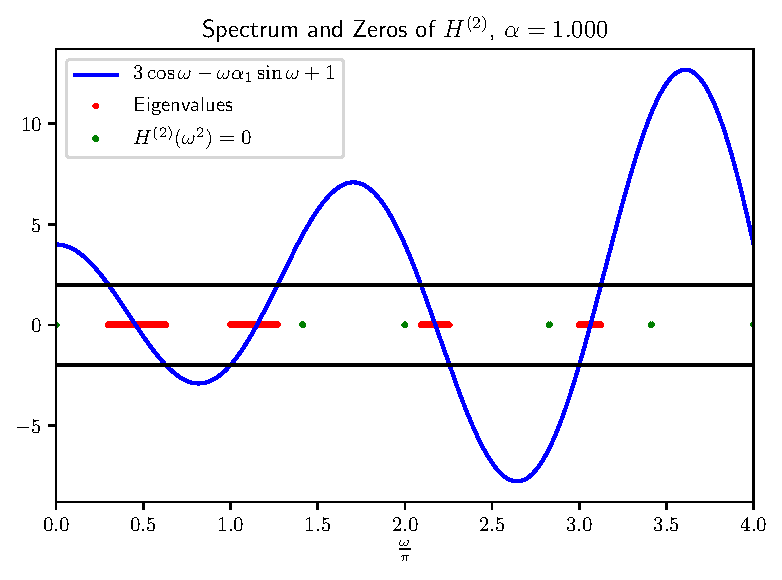
\includegraphics[scale=0.525]{1DDecoratedGraph_alpha1.pdf}
		\caption[]{\label{fig:1DDecoratedGraph_alpha1} The values of $\omega$ which solve \eqref{eq:EmbeddedGraphDetSolveCondition} with $\alpha_1=1$. No zeros of $H^{(2)}$ form part of the spectrum in this case.}
	\end{subfigure}
	~
	\begin{subfigure}[t]{0.45\textwidth}
		\centering
		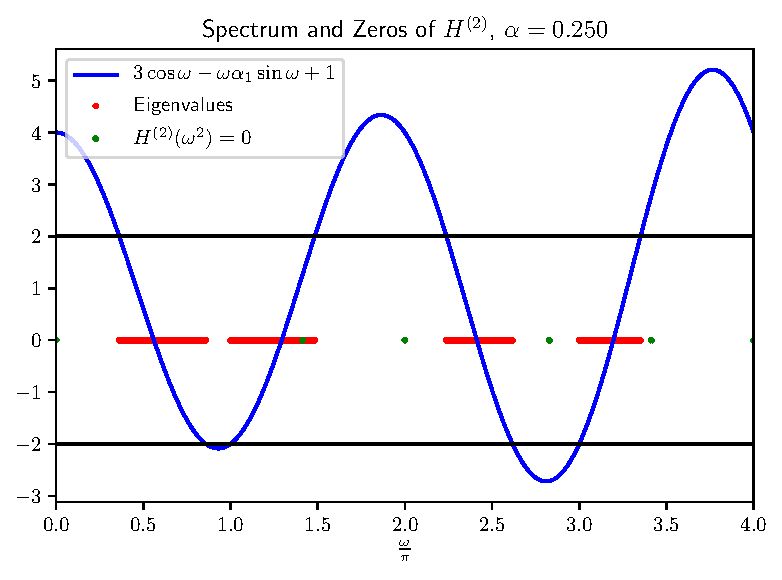
\includegraphics[scale=0.525]{1DDecoratedGraph_alpha0-25.pdf}
		\caption[]{\label{fig:1DDecoratedGraph_alpha0-25} The values of $\omega$ which solve \eqref{eq:EmbeddedGraphDetSolveCondition} with $\alpha_1=\recip{4}$. With $\alpha_1$ this small, some of the zeros of $H^{(2)}$ form part of the spectrum.}
	\end{subfigure}
	\caption[The spectrum of \eqref{eq:SingularScalarWaveEqn} on the geometry of section \ref{ssec:EmbeddingDependentExample}, and the corresponding poles of the determinant of the $M$-matrix.]{\label{fig:1DDecoratedGraph} The values of $\omega$ which solve \eqref{eq:EmbeddedGraphDetSolveCondition}, using $a=\recip{\sqrt{2}}$. Changing the value of $\alpha$ effects how many zeros of $H^{(2)}$ are included in the spectrum.}
\end{figure}

Zeros of $H^{(2)}$ occur at $\omega= 2n\pi, \frac{n\pi}{a}, \frac{n\pi}{1-a}$, but examining the limit \eqref{eq:EigenvalueBranchLimit} reveals that if $H^{(2)}\bracs{\omega_0^2}=0$, $\omega_0$ is part of the spectrum only when there exists a $\qm_0\in\left[-\pi,\pi\right)$ such that $\Xi\bracs{\omega_0}=\cos\theta_0+\recip{2}$.
That is, we once again require $F\bracs{\qm,\omega}=0$ for a root of $H^{(2)}$ to be part of the spectrum.
It is also worth noting that (in figure \ref{fig:1DDecoratedGraphEvalBranches-Thetas}) there are two eigenvalue branches $\widetilde{\beta}_j^{\qm}$ which are zero at $\omega_0$ (the third being non-zero at $\omega_0$).
The limit \eqref{eq:EigenvalueBranchLimit} exists for both branches, however only for one is it zero --- these branches and the corresponding limits in the vicinity of root $\omega_0=\pi\sqrt{2}$ are plotted in figure \ref{fig:1DDecoratedGraphEvalBranches-Thetas}.
\begin{figure}[t!]
	\centering
	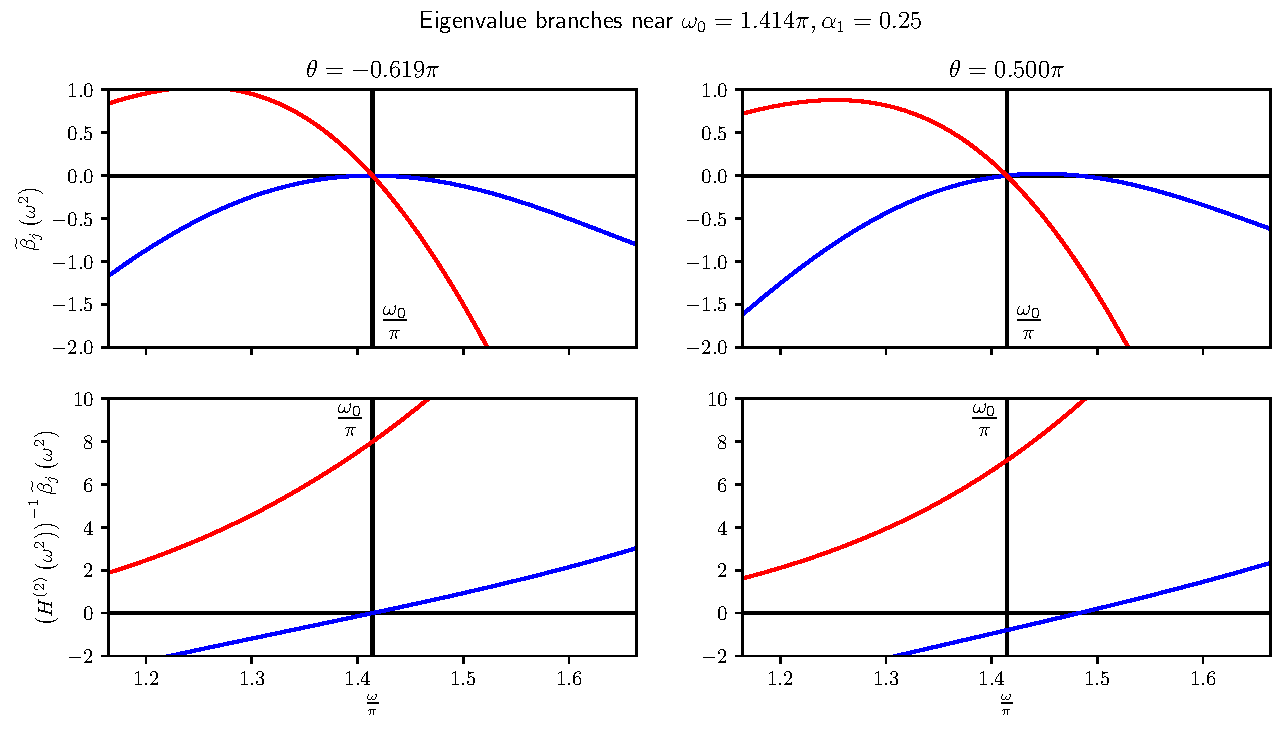
\includegraphics[width=\textwidth]{1DDecoratedGraphEvalBranches-Thetas.pdf}
	\caption[Eigenvalue branches of the $M$-matrix near a pole of the determinant, for the geometry of section \ref{ssec:EmbeddingDependentExample}.]{\label{fig:1DDecoratedGraphEvalBranches-Thetas} Eigenvalue branches of the matrix $\mathfrak{M}_{\qm}$ near $\omega_0 = \pi\sqrt{2}$, which is a root of $H^{(2)}$. The value $\qm_0\approx-0.691\pi$ solves $\Xi\bracs{\omega_0}=\cos\qm_0+\recip{2}$, and the limit \eqref{eq:EigenvalueBranchLimit} is zero. For all other values of $\qm$ however, the limit \eqref{eq:EigenvalueBranchLimit} is non-zero.}
\end{figure}

In summary, $\sigma$ consists of those $\omega^2$ such that
\begin{align*}
	\abs{ 3\cos\omega - \alpha_1\omega\sin\omega + 1 } \leq 2,
\end{align*}
which again is precisely those $\omega$ such that there is some $\qm$ such that $\bracs{\qm,\omega}\in F^{-1}\bracs{\clbracs{0}}$.
As expected, the spectrum does not depend on $\beta$ despite the fact that the $M$-matrix for each operator on $\graph^*$ does.
The spectrum differs from the spectrum of the quantum graph in section \ref{ssec:Example1DLoop} due to the presence of the ``decoration" $I_{12}$, although this difference only\footnote{If the coupling constant were non-zero, it would of course depend on this value too.} depends on the length of the decorating edge. This can be attributed to the graphs $\graph$ for every angle $\beta$ being a realisation of the same abstract quantum graph $\graph_{\mathcal{Q}}$, the problem on which can only depend on the lengths assigned to each of the edges.

\subsection{Cross-in-the-plane geometry} \label{ssec:ExampleCrossInPlane}
Our final example is a two-dimensional graph whose period cell represents a lattice-like structure in $\reals^2$.
Consider the embedded, periodic graph $\hat{\graph}$ defined as follows --- for each $\bracs{n,m}\in\integers^2$ define
\begin{align*}
	v^{(n,m)} &= \bracs{n+\recip{2}, m+\recip{2}}, \quad
	I_{\mathrm{left}}^{\bracs{n,m}} = \sqbracs{v^{\bracs{n,m}}, v^{\bracs{n+1,m}}}, \quad
	I_{\mathrm{up}}^{\bracs{n,m}} = \sqbracs{v^{\bracs{n,m}}, v^{\bracs{n,m+1}}}, \\
	\hat{\vertSet} &= \clbracs{v^{\bracs{n,m}} \setVert \bracs{n,m}\in\integers^2}, \quad
	\hat{\edgeSet} = \clbracs{ I_{\mathrm{l}}^{\bracs{n,m}}, I_{\mathrm{u}}^{\bracs{n,m}} \setVert \bracs{n,m}\in\integers^2}, \quad
	\hat{\graph} = \bracs{\hat{\vertSet}, \hat{\edgeSet}}.
\end{align*}
Place a coupling constant $\alpha^{\bracs{n,m}} =: \alpha_3>0$ at each $v^{(n,m)}$.
The period graph $\graph$ occupies $\left[0,1\right)^2$ and consists of a single vertex with two looping edges of length 1.
Breaking the loops by introducing two artificial vertices takes us to the quantum graph
\begin{align*}
	\vertSet^* = \clbracs{v_1, v_2, v_3}, \quad
	\edgeSet^* = \clbracs{I_{13}, I_{31}, I_{23}, I_{32}}, \quad
	\graph^* = \bracs{\vertSet^*, \edgeSet^*},
\end{align*}
with
\begin{align*}
	l_{13} = b, \quad l_{31} = \tilde{b} := 1-b, \quad 
	l_{23} = a, \quad l_{32} = \tilde{a} := 1-a, \qquad
	\qm_{13} = \qm_{31} = \qm_2, \quad \qm_{23} = \qm_{32} = \qm_1,
\end{align*}
and coupling constant $\alpha_3$ at $v_3$ (and zero coupling constants at the dummy vertices $v_1$ and $v_2$).
Using corollary \ref{cory:M-MatrixEntriesNoPoles} we set $H^{(2)}\bracs{\omega^2} = s_a\bracs{\omega} s_b\bracs{\omega} \tilde{s}_a\bracs{\omega} \tilde{s}_b\bracs{\omega}$, and obtain
\begin{align*}
	\mathfrak{M}_{\qm} & \bracs{\omega^2} = \\
	&
	\begin{pmatrix}[2.5]
		-\omega s_a \tilde{s}_a \bracs{ s_b \tilde{c}_b + c_b \tilde{s}_b } &
		0 &
		\begin{split}
			&\omega s_a \tilde{s}_a \bracs{ e^{\rmi\qm_2\tilde{b}}s_b + e^{-\rmi\qm_2 b}\tilde{s}_b }
		\end{split} \\
		0 &
		-\omega s_b \tilde{s}_b \bracs{ s_a \tilde{c}_a + c_a \tilde{s}_a } &
		\begin{split}
			&\omega s_b \tilde{s}_b \bracs{ e^{\rmi\qm_1\tilde{a}}s_a + e^{-\rmi\qm_1 a}\tilde{s}_a } 
		\end{split} \\
		\omega s_a \tilde{s}_a \bracs{ e^{-\rmi\qm_2\tilde{b})}s_b + e^{\rmi\qm_2 b}\tilde{s}_b } &
		\omega s_b \tilde{s}_b \bracs{ e^{-\rmi\qm_1\tilde{a}}s_a + e^{\rmi\qm_1 a}\tilde{s}_a } &
		\begin{split}
			&-\omega ( s_a s_b \tilde{s}_a \tilde{c}_b 
			+ s_a s_b \tilde{c}_a \tilde{s}_b \\ 
			& + s_a c_b \tilde{s}_a \tilde{s}_b
			+ c_a s_b \tilde{s}_a \tilde{s}_b \\
			& - \omega\alpha_3 s_a s_b \tilde{s}_a \tilde{s}_b )
		\end{split}
	\end{pmatrix}.
\end{align*}

Examining \eqref{eq:QGDetSolveCondition} yields
\begin{align} \label{eq:ExampleThickVertexSolution}
	0 = \omega^3 \bracs{H^{(2)}\bracs{\omega^2}}^2 \tilde{s}_b^2\bracs{\omega} \sin\bracs{\omega} 
	\bracs{ 4\cos\bracs{\frac{\qm_1+\qm_2}{2}}\cos\bracs{\frac{\qm_1-\qm_2}{2}} + \omega\alpha_3\sin\omega - 4\cos\omega }
\end{align}
although for ease we also define
\begin{align*}
	\Xi\bracs{\omega} := \cos\omega - \frac{\alpha_3\omega}{4}\sin\omega.
\end{align*}
Note that any $\omega_0$ for which $-1\leq\Xi\bracs{\omega_0}\leq 1$, there is some $\qm_0$ such that the bracketed factor in \eqref{eq:ExampleThickVertexSolution} is zero --- this again encompasses the case when $\sin\omega=0$, as in this case $\Xi\bracs{\omega} = \pm 1$.
Examination of the eigenvalue branches then produces a familiar conclusion; if $H^{(2)}\bracs{\omega_0^2}=0$, $\omega_0$ forms part of the spectrum of \eqref{eq:SingularWaveEqnQGProblem} if and only if there exists a $\qm_0$ such that
\begin{align} \label{eq:ExampleThickVertexSolutionReduced}
	\Xi\bracs{\omega}=\cos\bracs{\frac{\qm_1+\qm_2}{2}}\cos\bracs{\frac{\qm_1-\qm_2}{2}},
\end{align}
that is when $F\bracs{\qm_0,\omega_0}=0$.
As a result, the spectrum consists of exactly those $\omega$ such that
\begin{align*}
	-1 \leq \cos\omega - \frac{\alpha_3\omega}{4}\sin\omega \leq 1.
\end{align*}
If $\alpha_3=0$, we observe that the spectral bands touch and there are no spectral gaps.
By introducing (geometric) contrast through the coupling constants, gaps between the spectral edges open.
For any $\alpha_3>0$, the spectral bands $I_n$ satisfy $I_n\subset\sqbracs{(n-1)\pi, n\pi}$, each with left-endpoint $(n-1)\pi$ and a right-endpoint strictly less than $n\pi$.
This behaviour is reversed for $\alpha_3<0$, the bands having right-endpoint $n\pi$ and left-endpoint strictly greater than $(n-1)\pi$.
For $\alpha\leq-2$ there is even a gap between an isolated eigenvalue at $0$ and the beginning of the band $I_1$ --- this provides us with a case where the inclusion $\overline{F_0\setminus H_0}\subset\sigma$ in corollary \ref{cory:ScalarSetInclusions} is strict.
However as mentioned in section \ref{sec:TP-DomainSetup} and the interpretation of the coupling constants in light of section \ref{sec:ScalarDerivation}, $\alpha<0$ does not correspond to any physical material.

In addition to recovering the spectrum of \eqref{eq:SingularWaveEqnQGProblem}, we can use \eqref{eq:ExampleThickVertexSolution} and \eqref{eq:QGGenEvalSolveNoPoles} to recover the eigenfunctions too.
For a given $\qm$, equation \eqref{eq:ExampleThickVertexSolutionReduced} can be solved for (a solution) $\omega=\omega_0$ (of course, we could instead choose an eigenvalue $\omega$ and compute the corresponding quasi-momentum for which $\omega\in\sigma_{\qm}$).
This $\omega_0$ corresponds to an eigenvalue $\omega_0^2$ of \eqref{eq:SingularWaveEqnQGProblem}, but also implies that there exists a $w\in\complex^{\abs{\vertSet}}$ such that \eqref{eq:QGGenEvalSolveNoPoles} holds at $\omega=\omega_0$.
We can compute the eigenvector(s) $w\in\complex^{\abs{\vertSet}}$ of $\mathfrak{M}_{\qm}\bracs{\omega_0^2}$ corresponding to its zero eigenvalue.
Identifying $w = \dmap u$ as the Dirichlet data of the eigenfunction $u$, and given \eqref{eq:EdgeEqnGeneralSolution}, the edge functions $u^{(jk)}$ can be obtained.
Some examples of the result of this process are plotted in figure \ref{fig:CrossInPlane-EdgePlot}; one can observe continuity of the eigenfunctions at the central vertex, whilst their incoming derivatives adhere to the Wentzell condition.
\begin{figure}[t!]
	\centering
	\begin{subfigure}[t]{0.45\textwidth}
		\centering
		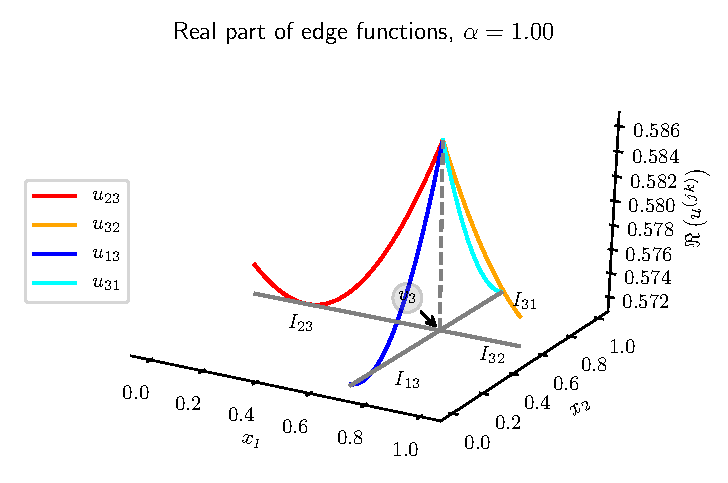
\includegraphics[width=\textwidth]{CrossInPlane_EdgePlot-R-a1.pdf}
		\caption[]{\label{fig:CrossInPlane_EdgePlot-R-a1} The real part of the eigenfunction corresponding to $\omega_0=0.63936, \alpha=1$.}
	\end{subfigure}
	~
	\begin{subfigure}[t]{0.45\textwidth}
		\centering
		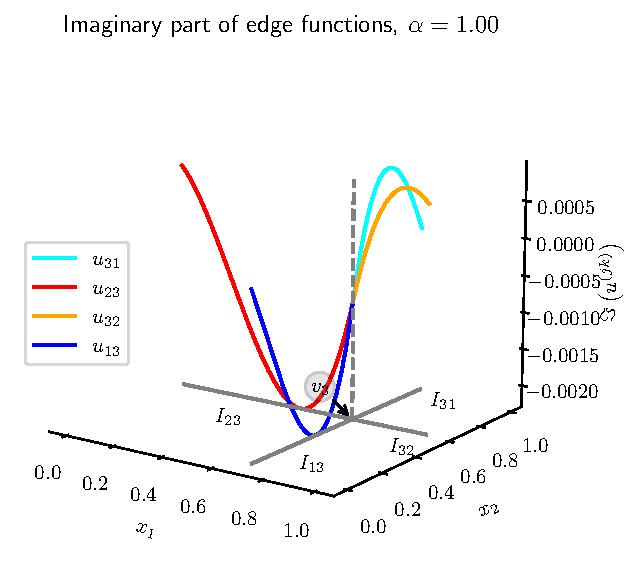
\includegraphics[width=\textwidth]{CrossInPlane_EdgePlot-I-a1.pdf}
		\caption[]{\label{fig:CrossInPlane_EdgePlot-I-a1} The imaginary part of the eigenfunction corresponding to $\omega_0=0.63936, \alpha=1$.}
	\end{subfigure}
	\vskip\baselineskip
	\begin{subfigure}[t]{0.45\textwidth}
		\centering
		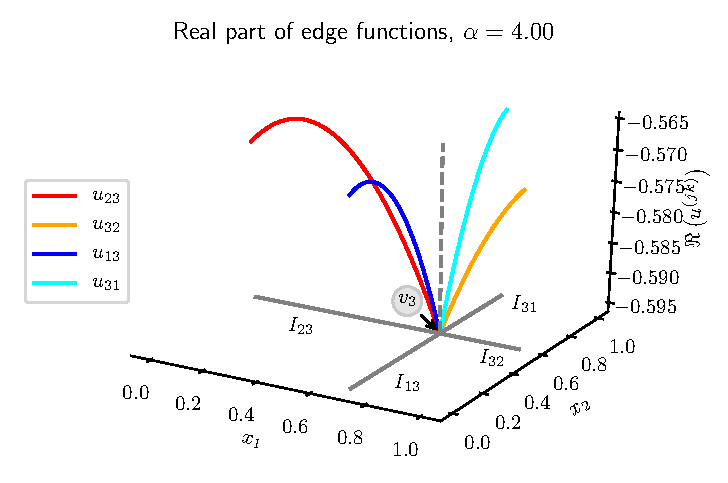
\includegraphics[width=\textwidth]{CrossInPlane_EdgePlot-R-a4.pdf}
		\caption[]{\label{fig:CrossInPlane_EdgePlot-R-a4} The real part of the eigenfunction corresponding to $\omega_0=0.44812, \alpha=4$.}
	\end{subfigure}
	~
	\begin{subfigure}[t]{0.45\textwidth}
		\centering
		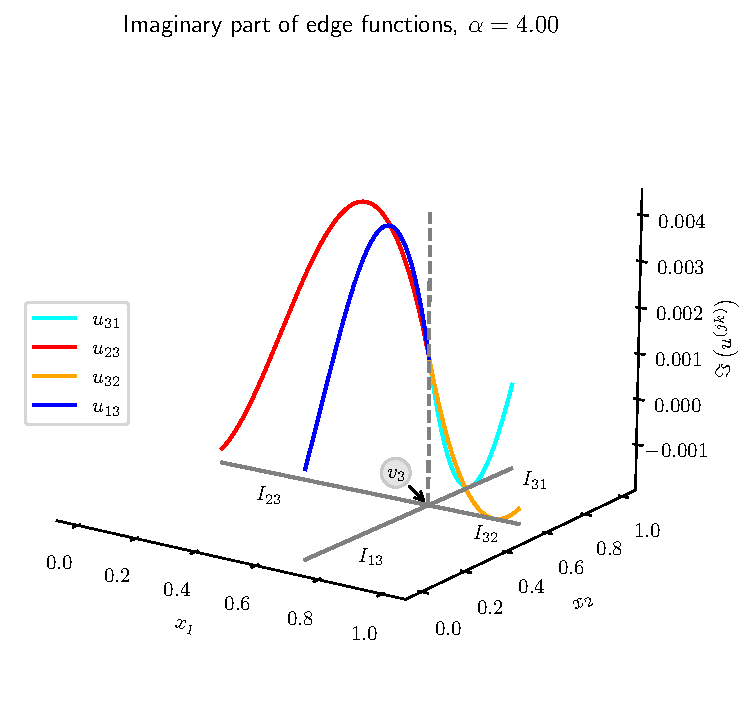
\includegraphics[width=\textwidth]{CrossInPlane_EdgePlot-I-a4.pdf}
		\caption[]{\label{fig:CrossInPlane_EdgePlot-I-a4} The imaginary part of the eigenfunction corresponding to $\omega_0=0.44812, \alpha=4$.}
	\end{subfigure}	
	\caption[Eigenfunctions of \eqref{eq:SingularScalarWaveEqn} on the cross-in-the-plane geometry.]{\label{fig:CrossInPlane-EdgePlot} Plots of the eigenfunctions corresponding to the eigenvalue $\omega_0=0.63936$  when $\alpha=1$, and $\omega_0=0.44812$ when $\alpha=4$. Both eigenvalues are attained when $\qm=\bracs{\frac{\pi}{4},\frac{\pi}{4}}^\top$, and the edge functions are plotted above the graph $\graph$ in the $\bracs{x_1,x_2}$-plane. We observe the expected continuity at the vertices, adherence to the Wentzell condition at $v_3$, and matching derivatives at the artificial vertices used to split the edges.}
\end{figure}
At the artificial vertices, we have matching of the incoming edge functions \emph{and} their derivatives, consistent with the zero coupling constant placed at dummy vertices.
To round off the analysis, quantities such as the integrated density of states (IDoS) and density of states (DoS) can also be estimated from \eqref{eq:ExampleThickVertexSolution}, as shown in figure \ref{fig:CrossInPlane_ScalarDoS} along with a display of the band-gap structure of the spectrum.
\begin{figure}[t!]
	\begin{subfigure}[t]{0.45\textwidth}
		\centering
		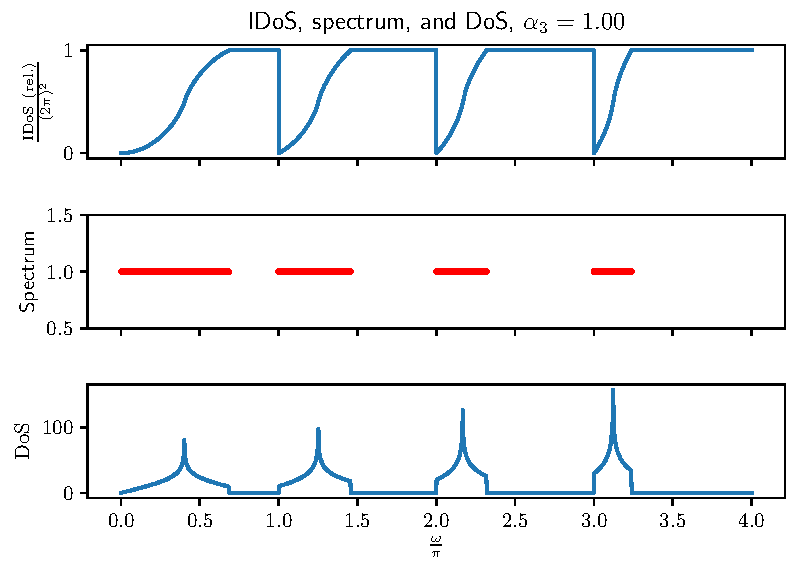
\includegraphics[scale=0.5]{CrossInPlane_ScalarDoS_alpha1-00.pdf}
		\caption[]{\label{fig:CrossInPlane_ScalarDoS_alpha1-00} The (relative) integrated density of states (IDoS), density of states (DoS) and spectrum for the system with $\alpha_3=1$.}
	\end{subfigure}
	~
	\begin{subfigure}[t]{0.45\textwidth}
		\centering
		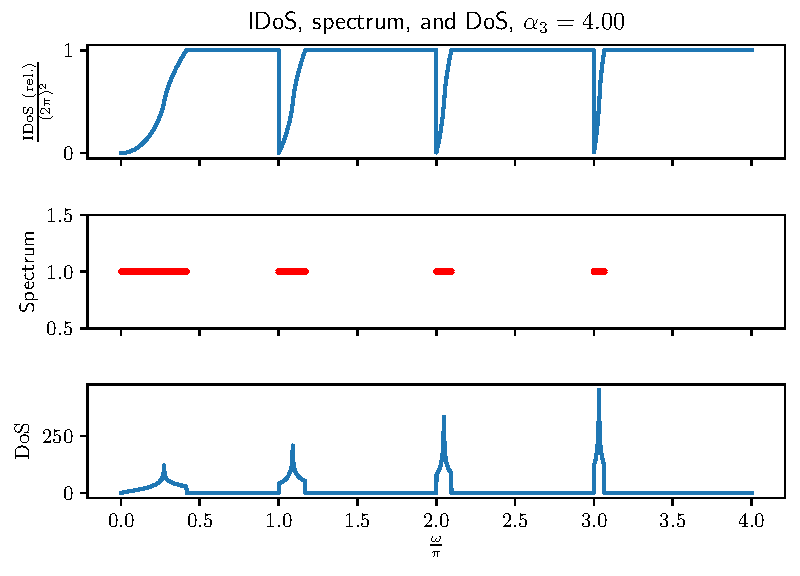
\includegraphics[scale=0.5]{CrossInPlane_ScalarDoS_alpha4-00.pdf}
		\caption[]{\label{fig:CrossInPlane_ScalarDoS_alpha4-00} The (relative) integrated density of states (IDoS), density of states (DoS) and spectrum for the system with $\alpha_3=4$.}
	\end{subfigure}	
	\caption[The spectrum and density of states for the problem \eqref{eq:SingularScalarWaveEqn} on the cross-in-the-plane geometry.]{\label{fig:CrossInPlane_ScalarDoS} The (relative) IDoS, DoS, and spectrum for the graph topology in section \ref{ssec:ExampleCrossInPlane}.
	The relative IDoS at the value $x$ is defined as the IDoS at the value $x$ minus $\left\lfloor\frac{x}{\pi}\right\rfloor\bracs{2\pi}^2$.}
\end{figure}
We observe that the spectrum concentrates in the centre of each band, as is to be expected from the symmetry of the geometry.